\documentclass{standalone}

\usepackage{../core}


\begin{document}
\begin{tikzpicture}
\node[inner sep=0pt] at (-2,-1) {
\includegraphics[width=4in]{bottleneck_col.pdf}};
\node[text=textcolor] at (-2,0.5) {\LARGE$\Omega$};
\node[text=textcolor] at (-4.8,-1) {\LARGE$\Omega_1$};
\node[text=textcolor] at (0.9,-1) {\LARGE$\Omega_2$};

\node[text=textcolor] at (-0.7,2.5) {\huge Decomposition theorem \qcite[\large]{Jerrum et al., '04}};

\node[text=textcolor] at (10.3,5) {\LARGE Projection chain};
\node[inner sep=0pt] at (10.2,3.5) {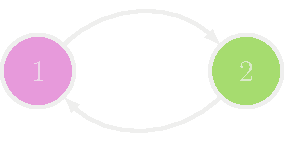
\includegraphics[width=1.5in]{projection.pdf}};

\node[textcolor] at (13.5,3.9) {\LARGE Gibbs};
\node[inner sep=0pt] at (14.7,3.85) {
\includegraphics[width=0.2in]{cross_mark_white.png}};
\node[textcolor] at (13.5,3.1) {\LARGE $\mathrm{M}^3$};
\node[inner sep=0pt] at (14.7,3.1) {
\includegraphics[width=0.2in]{check_mark_white.png}};

\node[text=textcolor] at (10.3,-1) {\LARGE Restriction chains};
\node[inner sep=0pt] at (10.2,-3) {
\includegraphics[width=1.3in]{bottleneck_col_left.pdf}};
\node[inner sep=0pt] at (10.2,-5.8) {
\includegraphics[width=1.3in]{bottleneck_col_right.pdf}};
\node[text=textcolor] at (10.0,-3.02) {\Large$\Omega_1$};
\node[text=textcolor] at (10.55,-5.8) {\Large$\Omega_2$};

\node[textcolor] at (13.5,3.9-7.8) {\LARGE Gibbs};
\node[inner sep=0pt] at (14.7,3.9-7.8) {
\includegraphics[width=0.2in]{check_mark_white.png}};
\node[textcolor] at (13.5,3.1-7.8) {\LARGE $\mathrm{M}^3$};
\node[inner sep=0pt] at (14.7,3.1-7.85) {
\includegraphics[width=0.2in]{cross_mark_white.png}};

\node[] (1) at (3.5,-1) {};
\node[] (2) at (7.5,3) {};
\node[] (3) at (7.5,-4.5) {};
\draw [-latex,line width=2.5pt,color=textcolor,line cap=round] (1) to[out=0,in=200] (2);
\draw [-latex,line width=2.5pt,color=textcolor,line cap=round] (1) to[out=0,in=160] (3);
\end{tikzpicture}
\end{document}